\chapter{Analýza}

\begin{chapterabstract}
Tato kapitola...
\end{chapterabstract}

\section{Aplikace na tvorbu prezentací}

Nejzákladnějším prvkem výuky je podpora toho, co učitel prezentuje před skupinou vyučovaných, a to tedy prezentace. 
Prezentace slouží jako doprovod k tomu, aby se neztratil jak učitel, tak i student. 
Pro tvorbu prezentaci existuje řada nástrojů a v této podkapitole zmíním ty nejvíce důležité pro mojí budoucí práci.

\subsection{PowerPoint}

PowerPoint je aplikace pro tvorbu prezentací z balíčků nástrojů Microsoft Office. 
PowerPoint je považován za standard pro tvorbu prezentací a skoro každý, kdo používá počítač by s ním měl umět.

Mezi hlavní výhody aplikace patří jeho obecnost a jednoduchost -- hodí se na všechno. 
Skvěle spolupracuje s ostatními MS Office aplikacemi, jako je Word či Excel. 

Uživatelé často jako nevýhody PowerPoint uvádějí problémy s kompatibilitou mezi verzemi a tím, jako moc obecný nástroj je a že jeho nástroje omezují kreativitu. 
Prezentace jsou taktéž často velmi limitovaně interaktivní a vede to hodně k pasivitě publika.

Prezentace je možné tvořit i prezentovat přímo na webové aplikaci, která dovoluje i spolupráci mezi více autory, avšak tato verze je řádně omezena funkcionalitami.
A to i když obě dvě verze jsou placené, což je nejvíce zmiňovaná nevýhoda této aplikace.

\subsection{Google Slides}

Slides od společnosti Google je webový nástroj pro tvorbu prezentací. Původně vznikal jako alternativa zdarma od společnosti Google. 

Výhody stojí zejména na tom, že služby Google Suite jsou stavěny na jednoduchou spolupráci mezi lidmi. 
Aplikace podporuje řadu funkcionalit stejně, jako PowerPoint. 
Limitace jsou však zřejmé, zejména z toho důvodu, že PowerPoint je k dispozici již přes~30 let. Naopak Google Slides jen něco přes 10~let. 
Zejména se pak konkrétně jedná o specifické formátování, možnosti vložení, animace a další.

\subsection{RevealJS}

RevealJS je knihovna a framework, která dovoluje tvořit prezentace za pomocí zdrojového kódu v \texttt{HTML}. 
Výsledné prezentace jsou k dispozici jako webová stránka, ve které se vykreslují jednotlivé snímky, mezi kterými lze procházet. 

Velkou výhodou RevealJS je jeho velká komunita a řada pluginů, které pohání připravené \texttt{API}. 
Celý projekt a i většina pluginů je open-source a díky pohánění na webu skoro neexistuje limit toho, co jde do prezentace vložit; ať se už jedná o videa, animace, kód ale i například jeho spouštění. 
Nevýhodou komunitního množství pluginů je různý způsob psaní kódu, dokumentace a nastavení, kdy jednotlivé pluginy nemusí být mezi sebou kompatibilní. 

Vytvořené prezentace musí být uloženy a k dispozici většinou na nějakém cloudovém místě autora prezentace, zejména pokud jsou používány pluginy, které například potřebují i mít k dispozici server.
Společnost, která vytvořila RevealJS poskytuje i službu Slides.com, ve které jde prezentace tvořit i pomocí editoru pomocí zmíněné knihovny.
Výhody této platformy je pak automatické cloudové uložení, prémiové pluginy (jako například automatické sledování přednášejícího) a již zmíněný editor. Platforma jako taková je potom i s prémiovými pluginy zcela closed-source.

Nevýhody celé této knihovny je právě způsob zápisu prezentace a to je \texttt{HTML}.
Sic je jazyk jednoduchý a velmi populární, není to pro každého a pro zcela správný sémanticky zápis je nutné spousta praxe a znalosti mimo.
Absence \texttt{WYSIWYG} tedy ztěžuje se do této knihovny ponořit.
Pro lepší design a celkové rozšíření je často nutné umět \texttt{CSS} a respektive \texttt{JS}.

Osobně RevealJS knihovnu již řadu let používám pro tvorbu prezentací pro studenty na střední škole.
Největší výhodu, což potvrzují i studenti, je to, že je možné v prezentaci tvořit interaktivní prvky.
V mém případě se jedná o kódový blok společně s okamžitým ukázáním výsledků, například na webových stránkách, jako je například vidět na obrázku \ref{fig:anaylza:revealjs-ukazka}.
Na jedné straně je kód, ve kterém studenti vidí zápis (který jde i prezentačně postupně ukazovat a měnit) a na druhé části vidí výsledek -- webovou stránku.

\begin{figure}[h!]
    \centering
    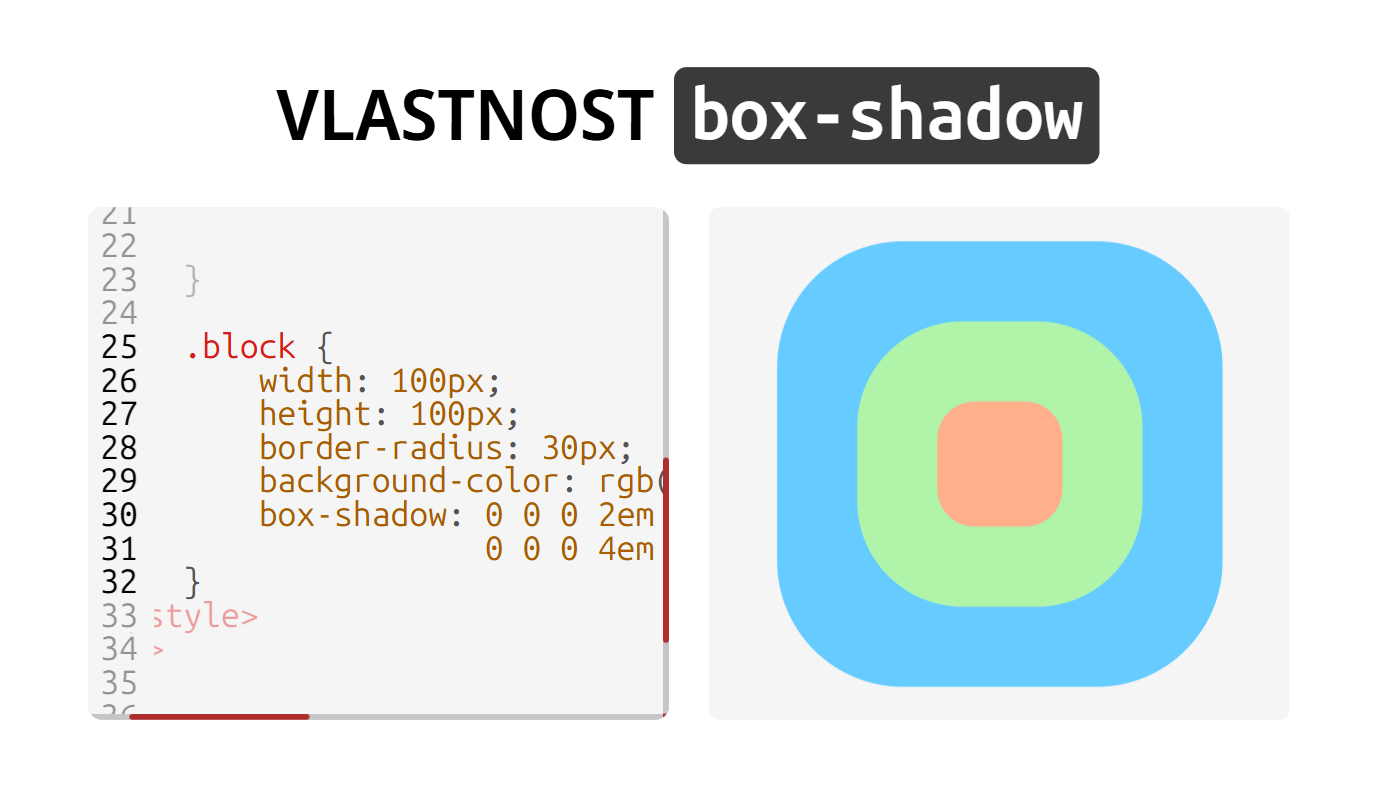
\includegraphics[width=0.9\linewidth]{media/03_analyza/revealjs.png}
    \caption{RevealJS prezentace s rozdělením kódu a výsledku}
    \label{fig:anaylza:revealjs-ukazka}
\end{figure}

Zajímavou funkcí ReavelJS jsou jejich takzvané \enquote{vertikální snímky}, kdy je možné místo klasického jednodimenzionálního průchodu tvořit postup takový, že prvně se preferuje pohyb dolů, a pokud již další snímek není v této mřížce k dispozici, tak do další \enquote{hromady} snímků vpravo. 
Celkově si lidi chválí i možnost modularity těchto snímků a že je velmi jednoduché spojovat jednotlivé atomické skupiny do větších celků.

\subsection{Beamer v \LaTeX}

Beamer je třída v sázecím systému \LaTeX, která se zaměřuje na vytváření snímkových prezentací.
Nejvíce je Beamer společně s \LaTeX~populární v akademickém prostředí zejména z důvodu jednoduchého sázení matematických formulí a zápisu pomocí kódového jazyka, který leccos dovoluje. 

Zápis je ale zároveň to nejvíce nenáviděné na \LaTeX, a to zejména z důvodu kryptických kódových chyb a různých zastaralých zápisů.
Vygenerované prezentace jsou taktéž statické a nedá se v nich dělat jakákoliv interaktivity. 
Výhodou takovéto kódové generace je, že často z jednoho zdrojového kódu -- pro prezentaci -- se dají tvořit taktéž skripta a to tím, že přidáváme takové bloky kódu, které vykreslí právě v jednom nebo v obou módech.

\section{Aplikace na grafickou tvorbu}

\subsection{Canva}

\subsection{Figma}

\section{Aplikace na tvorbu materiálů}

\subsection{Genially}

\subsection{Mentimeter}

\subsection{Prezi}

\section{Sumarizace knihoven a nástrojů}

Tabulka kde vse vyse uvedene nejak sumarizuji, co chybi

\section{Interaktivní prvky}

Podívat se jak fungují různé nástroje pro vzdělávání, interakce, např. hello-algo, kahoot, blooket

\section{Správa komunitních rozšíření}

Jak to resi google, revealjs ale i neco pokrocilejsiho, hlavne resit bezpecnost